\begin{figure}[H]
\begin{adjustwidth}{-\extralength}{0cm}
\centering
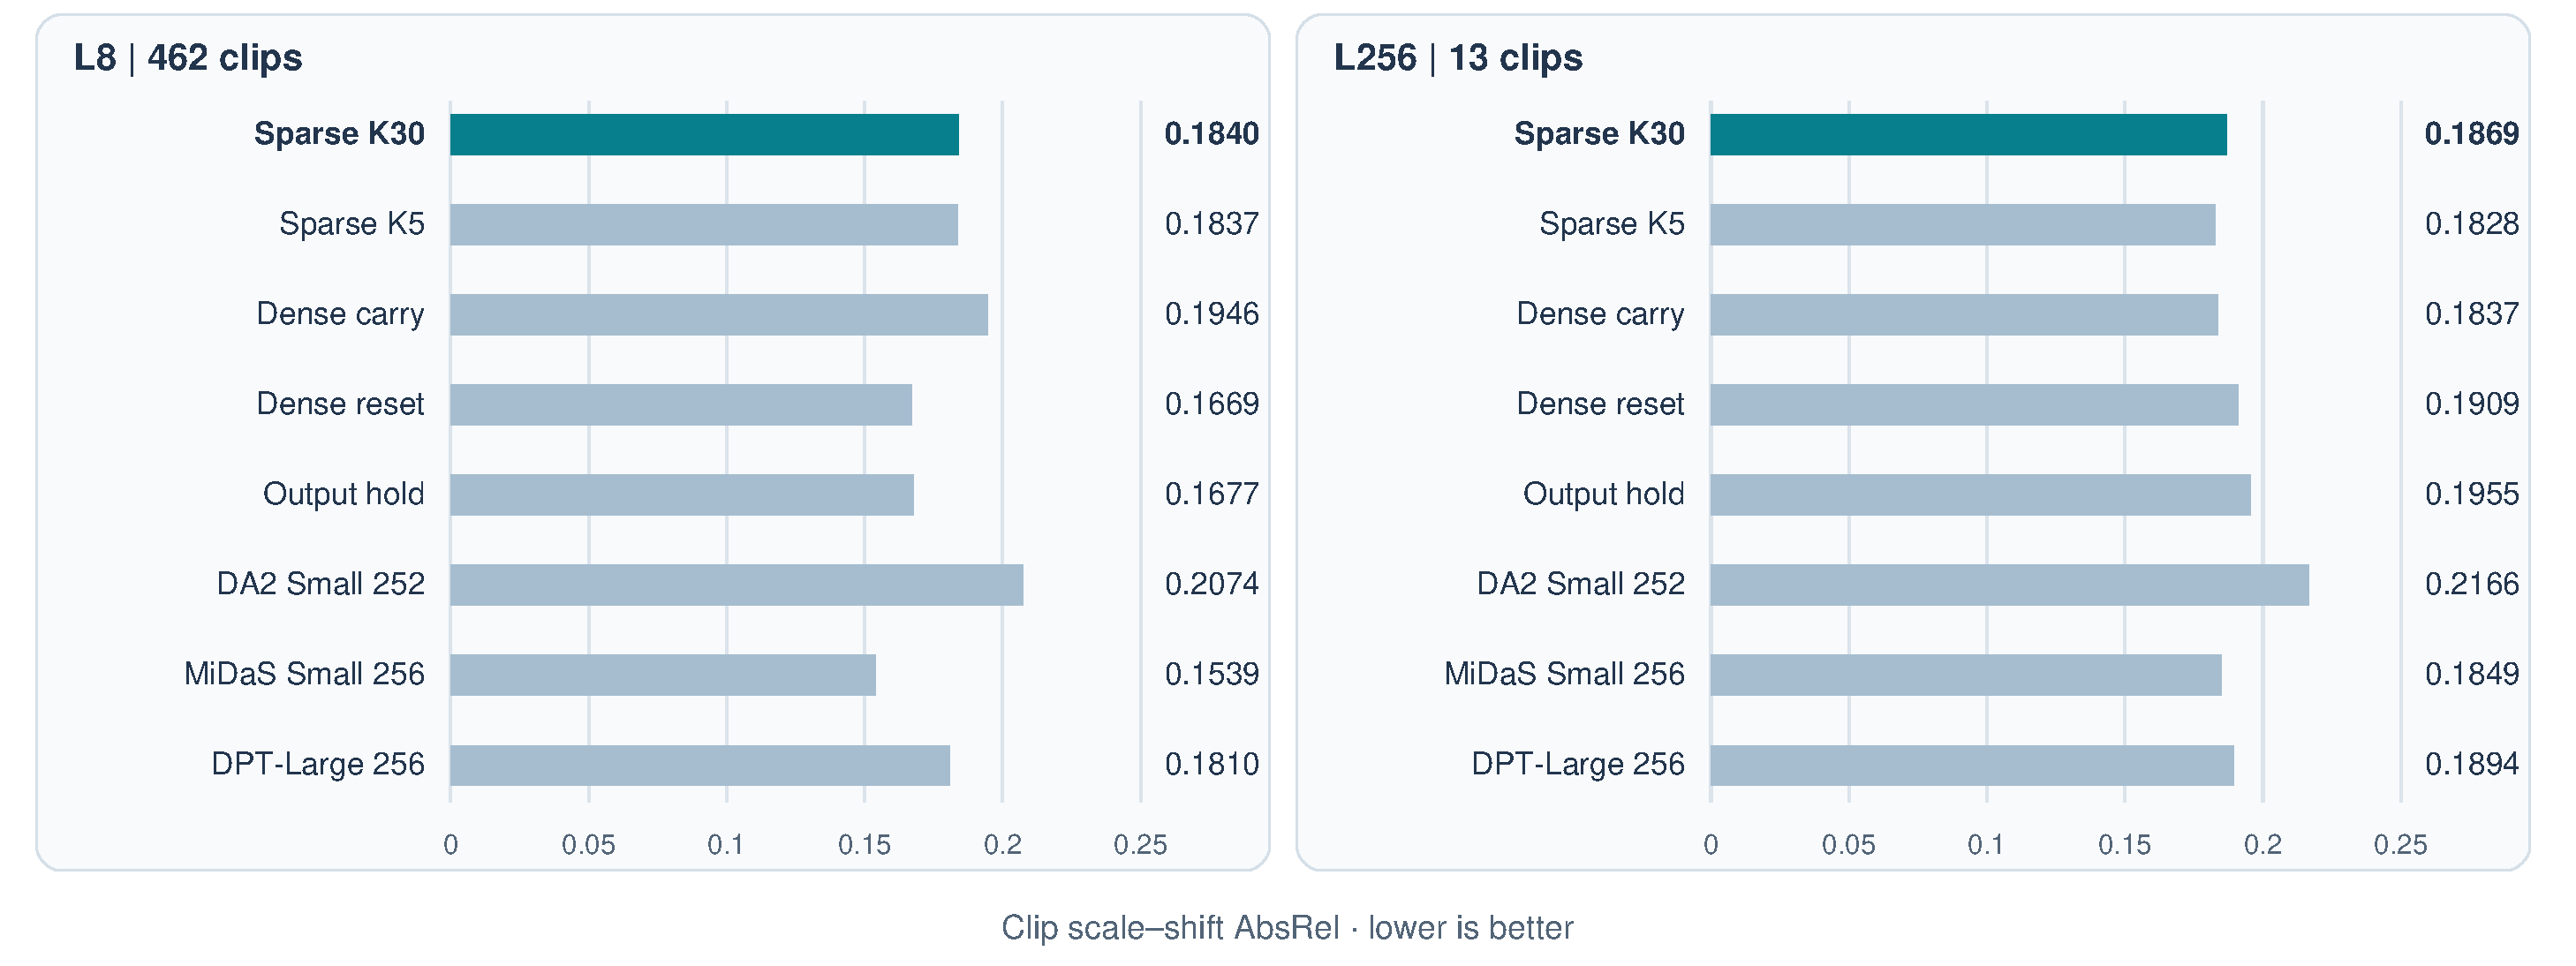
\includegraphics[width=\fulllength]{figures/r3_accuracy.pdf}
\caption{All eight frozen paths on L8 and L256, using the source pixel-pooled
clip scale--shift AbsRel estimator of the main tables. Zero-based axes and all
failed fits are retained. These point estimates have no sequence uncertainty
bars: the exploratory paired sequence estimator is reported separately.
The two lengths share some footage but are not identical history interventions.}\label{fig:accuracy}
\end{adjustwidth}
\end{figure}

\begin{figure}[H]
\begin{adjustwidth}{-\extralength}{0cm}
\centering
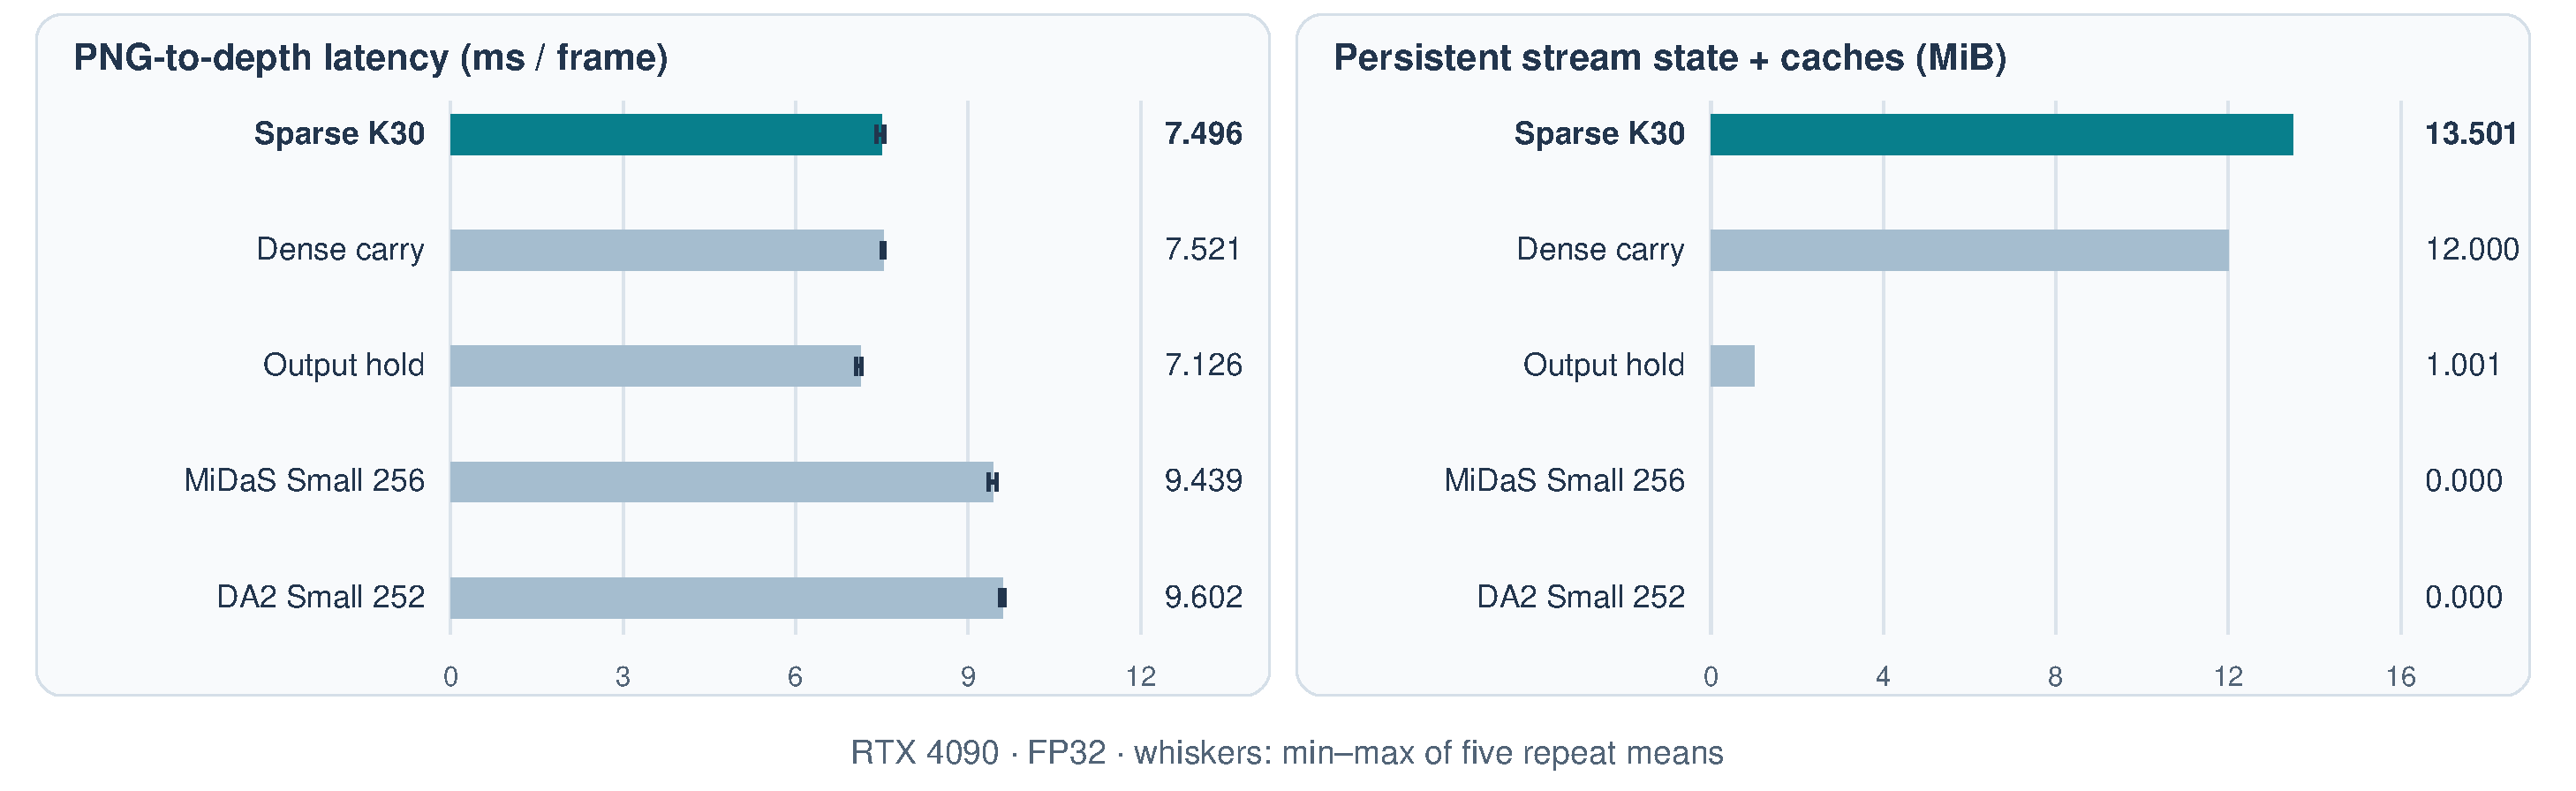
\includegraphics[width=\fulllength]{figures/r3_cost.pdf}
\caption{Development-only measured cost for five representative operating points.
Latency includes the same PNG-to-depth boundary on four matched L256 clips;
whiskers show the minimum/maximum of five repeat means, not confidence intervals.
Persistent stream memory excludes weights and transient buffers; zero state in
an image model does not mean zero total memory. Final-test accuracy is not used
to claim matched-quality acceleration.}\label{fig:cost}
\end{adjustwidth}
\end{figure}

\begin{figure}[H]
\begin{adjustwidth}{-\extralength}{0cm}
\centering
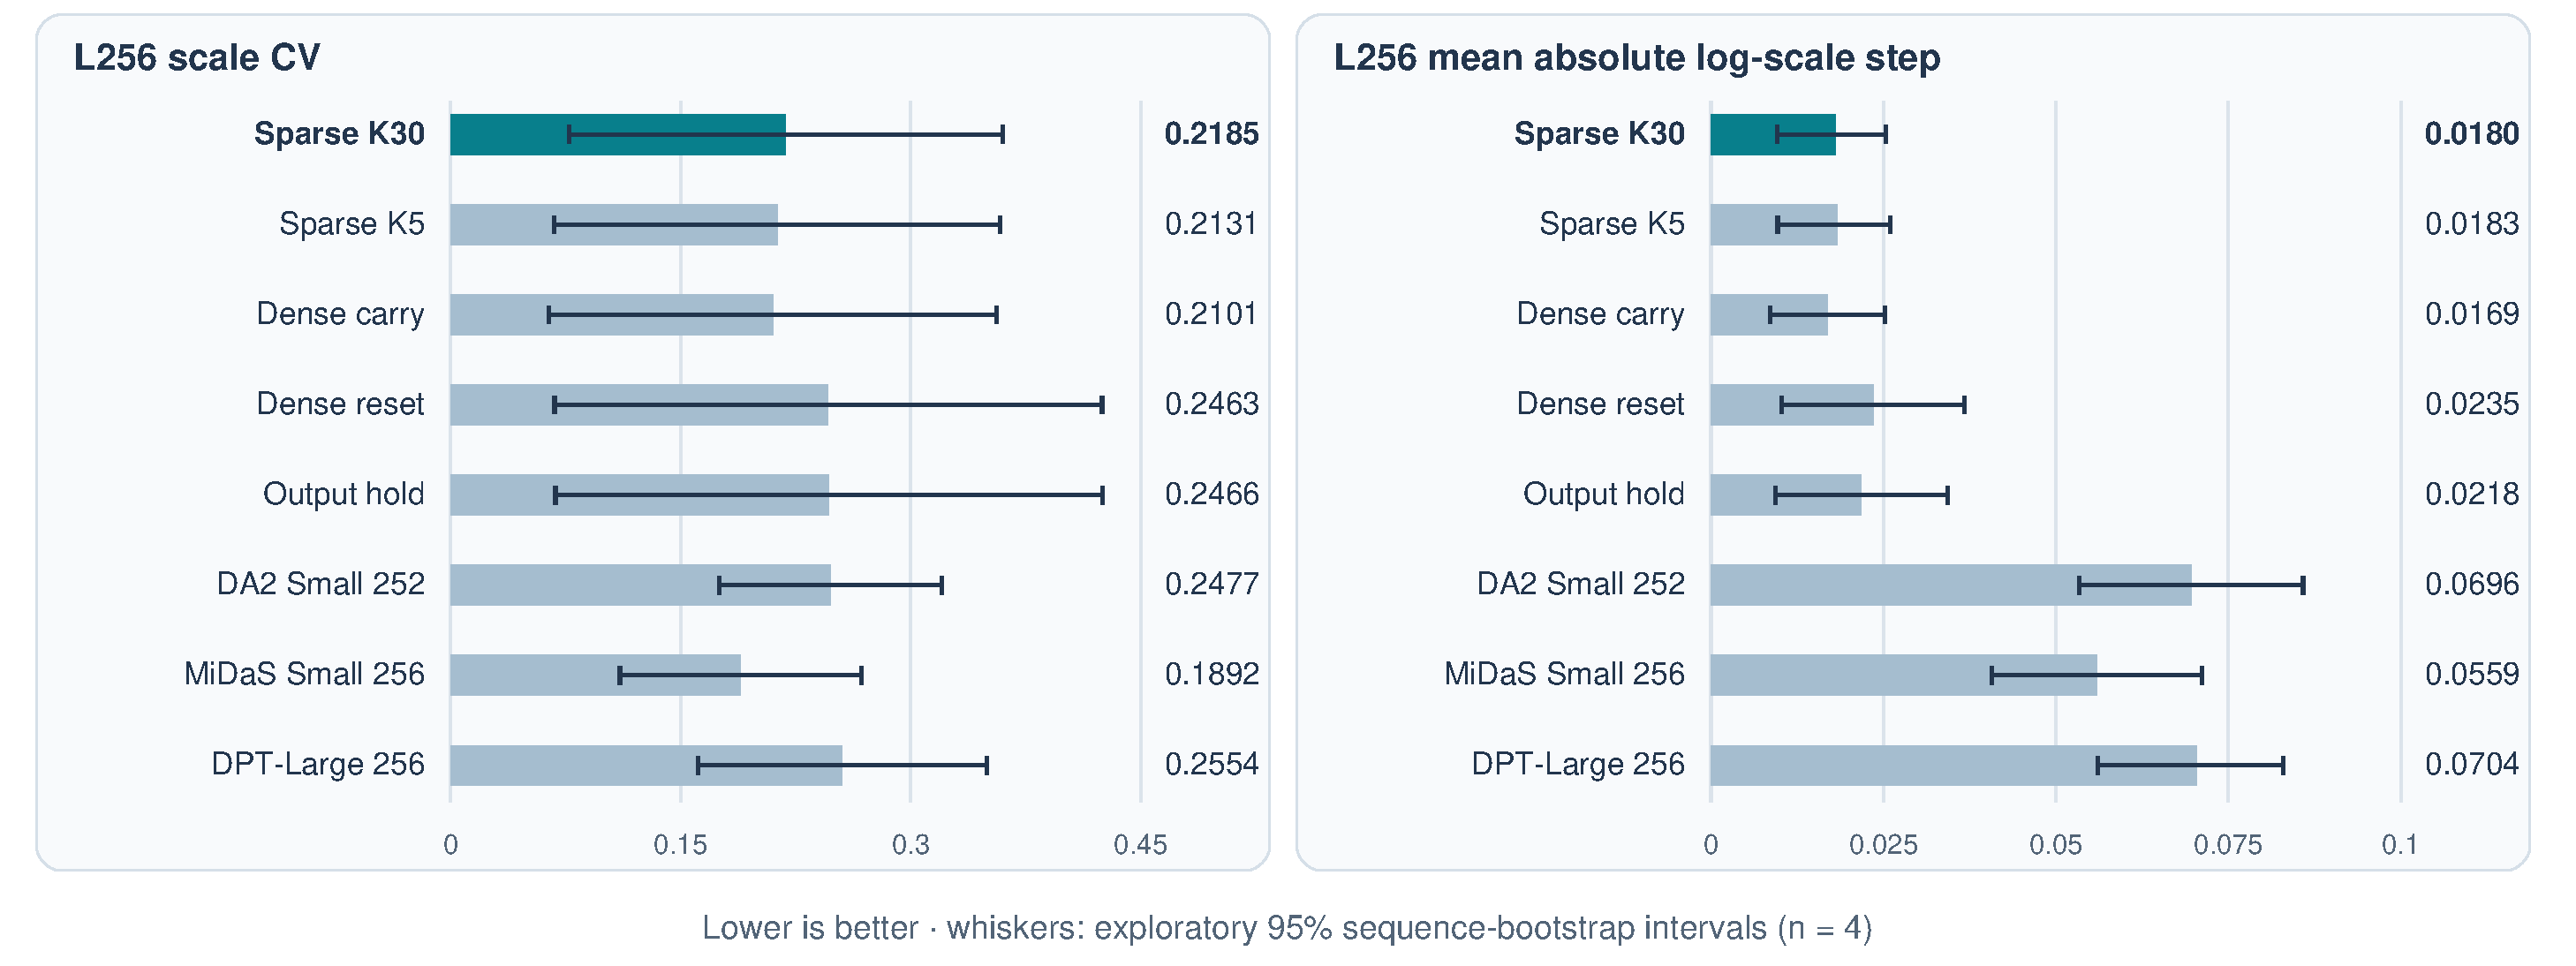
\includegraphics[width=\fulllength]{figures/r3_scale.pdf}
\caption{Post-hoc scale diagnostics for all eight frozen L256 paths. Four-sequence
means and exploratory, unadjusted percentile sequence-bootstrap intervals;
clip means are averaged within each sequence first. Native predictions use
no-fit depth, while relative predictions use median-gauge depth. CV describes
within-clip variation and log-step describes short-step variation; neither is
a substitute for depth accuracy or proof of general temporal superiority.}\label{fig:scale}
\end{adjustwidth}
\end{figure}
